%\part[Introdução]{Introdução}

\chapter{Introdução}

RFID (\textit{Radio Frequency Identification} ou Identificação por Rádio Freqüência) é uma tecnologia utilizada para identificar, rastrear e gerenciar desde produtos e documentos até animais ou mesmo indivíduos, sem contato e sem a necessidade de um campo visual.\cite{coe} Diversas situações comuns no dia a dia da população podem se tornar mais seguras ou ágeis com o uso da tecnologia de RFID, desde controles de acesso até gerenciamento de estoques.

Por não necessitar de contato manual, a força de trabalho que, em situações sem o uso de tecnologias de identificação, estaria ocupada realizando estas tarefas, pode dedicar seu tempo a outras atividades, tornando processos empresarias ou industriais muito mais eficientes.

Apesar de o RFID ter algumas funções similares às do código de barras, cada vez mais se comprova que o RFID, com suas etiquetas inteligentes, completa o código de barras. A perspectiva é que uma grande revolução na gestão da cadeia de suprimentos será proporcionada através da larga adoção de RFID, fornecendo informações em tempo real para o seu gerenciamento.\cite{coe}

Atualmente, procedimentos de identificação automática se tornaram populares em muitas empresas de serviços, logísticas de compra e distribuição, industria e manufaturas. Estes procedimentos existem para prover informações sobre pessoas, animais, bens e produtos em trânsito. \cite{Fink}

A presença universal de etiquetas de códigos de barra que proporcionou uma revolução nos sistemas de identificação algum tempo atrás está se tornando obsoleto em um número cada vez maior de situações. Apesar de serem baratos, sua baixa capacidade de armazenamento de dados e o fato de não serem reprogramados são pontos negativos. \cite{Fink}

As projeções futuras para este campo são extremamente motivadoras. A crescente necessidade de identificação imediata faz do uso dessa tecnologia algo não só preferível, como obrigatório para diversas aplicações.  Em um futuro cada vez mais conectado, onde as informações devem ser recebidas e processadas o mais rápido possível, e que o não processamento de ditas informações em tempo hábil podem ser a diferença entre o lucro ou o prejuízo de um negócio, ou a vida e a morte de um animal, a tecnologia RFID possui um potencial enorme para impactar o futuro da sociedade, tal como foi com outras tecnologias de identificação como o código de barras.

\section{Contextualização}

Em \cite{Roberta}, foi feita a modelagem de duas arquiteturas propostas para um sistema de RFID usando a linguagem SystemC e sua extensão SystemC-AMS. Com isso, foi possível verificar a funcionalidade de cada arquitetura através de simulações em alto nível de abstração, incluindo as partes analógicas e de RF.

Em \cite{Marlon}, os blocos constituintes do \textit{front-end} analógico de uma tag passiva de RFID para 13,56 MH, cujo diagrama de blocos está mostrado na Figura \ref{11}, foram desenvolvidos utilizando a linguagem Verilog-AMS. O projeto elétrico de um demodulador ASK foi realizado usando a tecnologia TSMC 0.18 um e utilizado em simulações mistas com os blocos descritos em Verilog-AMS. O layout do demodulador foi enviado para fabricação, juntamente com outros blocos individuais \cite{waamaral}.

\begin{figure}[h!]
  \centering
  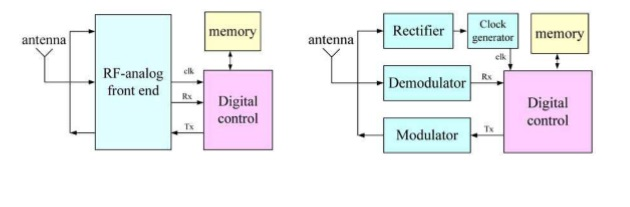
\includegraphics[width=0.8\textwidth]{blocos.jpg}
  \caption{Diagrama de blocos do sistema.\cite{li2009}}
  \label{11}
\end{figure}

A caracterização do demodulador e do \textit{bandgap} foi feita em \cite{jose}, juntamente com o projeto e layout dos blocos individuais restantes do \textit{front-end} analógico da tag. Para validar os circuitos projetados, foram realizadas simulações mistas entre blocos modelados em Verilog-AMS e esquemáticos em nível de transistores.

Por fim, para o projeto dos blocos digitais da tag, um protocolo anticolisão foi descrito em Verilog e simulado em \cite{henriq}, considerando que a comunicação entre o leitor e a \textit{tag} segue o protocolo ISO/IEC 14443 e que inicialmente a \textit{tag} enviará apenas o ID para o leitor, sendo que poderá ocorrer colisão de dados quando o leitor acionar mais de uma \textit{tag}.

\newpage
\section{Objetivo Geral}

Como continuação dos trabalhos anteriores a respeito do tema, este trabalho tem como objetivos gerais a verificação do sistema usando simulações mistas entre os blocos do \textit{front-end} analógico e os blocos digitais, bem como a preparação para síntese lógica e física dos blocos do controle digital da \textit{tag} passiva de RFID na frequência de 13,56MHz.

\section{Objetivos Específicos}

Para simular a \textit{tag} completa, os blocos descritos em Verilog-AMS e Verilog serão gradativamente adicionados. Após a validação, será realizada a preparação dos arquivos para a geração do layout dos blocos digitais, na tecnologia TSMC 0.18 um, utilizando ferramentas de síntese automática da Cadence. Sendo assim, os objetivos específicos são:

\begin{itemize}

\item Simulação mista do demodulador ASK com um bloco de memória;
\item Simulação mista do demodulador, memória e modulador;
\item Simulação mista do demodulador, memória, modulador e do bloco de controle digital;
\item Adaptação dos scripts de síntese para os arquivos da biblioteca da TSMC 0.18 um e para as ferramentas de síntese da Cadence;
\end{itemize}

\section{Estrutura do Trabalho}

O trabalho está dividido conforme a descrição a seguir. Inicialmente, é apresentada uma introdução geral ao tema, expondo a motivação, contextualização e os objetivos do trabalho. O Capítulo 2 contém uma fundamentação teórica sobre RFID, seus componentes e funcionamento. No Capítulo 3, é feito um estudo sobre projetos de circuitos integrados digitais, abordando o fluxo de projeto e ferramentas utilizadas. O Capítulo 4 contém a descrição da modelagem dos blocos digitais para a realização da simulação mista, e o Capítulo 5, os resultados da verificação. Por fim, o Capítulo 6 contém a conclusão, com considerações sobre os resultados obtidos e sugestões para trabalhos futuros. Como não foi possível realizar as sínteses lógica e física devido à falta de licença da ferramenta, a preparação dos arquivos e descrição dos passos necessários para gerar o layout se encontram no Apêndice A.

\section{Aspectos Metodológicos}

Este trabalho iniciou-se com uma revisão biblíográfica acerca da tecnologia de RF, suas aplicações e sistemas. Em seguida, fez-se necessária a realização de diversos tutoriais para a aprendizagem do uso das ferramentas de simulações. No caso de simulações mistas, o software utilizado foi o Virtuoso da Cadence. Por fim, foram buscados os arquivos de trabalhos anteriores contendo a descrição dos blocos de front-end analógico, e os resultados de simulação foram reproduzidos.

Após o domínio básico do software, foi realizada a modelagem dos blocos digitais para que fosse possível realizar as simulações mistas. Nessa etapa, foram modelados os blocos conversor serial-paralelo, memória e conversor paralelo-serial, tais como os sub-blocos que os compõem, através da metodologia top-down.

A última etapa consistiu em realizar as simulações dos blocos digitais isolados, realizar a conexão entre os blocos digitais e analógicos e por fim realizar as simulaçoes mistas. Para analisar os resultados das simulações, foram utilizados trabalhos anteriores no campo dos blocos analógicos para se entender o que deveria ser esperado das simulaçõse realizadas.